\documentclass[12pt]{article}
\usepackage[pdftex]{graphicx}
\usepackage{epstopdf}
\usepackage{amsmath, algorithmic, color, multicol}
\usepackage{subfigure}


\title{Answers to Problem Set 3}
\author{
	Lauren Hinkle (lhinkle)\\
	Pedro d'Aquino (pdaquino)\\
	Robert Goeddel (rgoeddel)}

\begin{document}
\maketitle
\pagebreak

%% TASK 1
\section{FastSLAM}

% PART A
\paragraph{A}
Starting with an existing EKF with state $\left[\begin{array}{c c c c c}x_0 & y_0 & t_0 & fx_0 & fy_0\end{array}\right]$ and a corresponding covariance matrix $\Sigma$.
\subparagraph{i}
For our first observation, we merely add our estimated position for the observation
directly to the mean/state vector based on our current position estimate and the
observation values $r$ and $\phi$. This gives us:

$$x' = \left[\begin{array}{c}x_0 \\
        y_0 \\
        \theta_0 \\
        fx_0 \\
        fy_0 \\
        x_0 + r * \cos (\theta_0 + \phi) \\
        y_0 + r * \sin (\theta_0 + \phi)
        \end{array}\right]
$$

To calculate the covariance, we need to base our uncertainties for our new observation
on the uncertainties of all we've seen before and the uncertainties introduced by taking
the observation itself. We use the formula:

$$\Sigma_w = \left[\begin{array}{c c}
    3 & 0 \\
    0 & 1 \end{array}\right]
$$

$$\Sigma'_x = J_x \Sigma_x J_x^T + J_w \Sigma_w J_w^T$$

In this case, $\Sigma_x$ is our old covariance and $\Sigma_w$ is our observational covariance.
$J_x$ is a $7 \times 5$ matrix in this case consisisting of the identity for the first 5 rows (preserving
the original entries) and then the jacobian of the observation equations $\frac{\delta r}{\delta x_0}$,
$\frac{\delta \phi}{\delta x_0}$, etc. for the initial state vector $x$. $J_w$ projects our covariance
from $(r,\phi)$ to $(x,y)$. $J_w$ is a $7 \times 2$ matrix in this case computed from our observation equations
used as seen in our initialization of $x'$. The result is a $7 \times 7$ covariance matrix.

\subparagraph{ii}
After re-observing $f_1$, the mean and covariance matrix are calculated using an updated Kalman gain (\emph{Note: additional primes denote
    later state}).
$$K' = \Sigma_x' J_{x'}^T(J_{x'} \Sigma_x' J_{x'}^T + \Sigma_z)^{-1} $$
$$x'' = x' + K'r'$$
$$\Sigma_x'' = (I - K'J_{x'}) \Sigma_x'$$

\subparagraph{iii}
After observing $f_1$: \\
$$\mu = \left[ \begin{array}{c}
3 \\
2 \\
pi \\
12 \\
15 \\
3 \\
-8
\end{array}\right],
\Sigma = \left[ \begin{array}{c c c c c c c}
4.00 & 1.00 & 2.00 & 1.00 & 1.00 & 1.00 & -2.40 \\
1.00 & 6.00 & 3.00 & 1.00 & 2.00 & 6.00 & -3.10 \\
2.00 & 3.00 & 4.00 & 1.00 & 2.00 & 3.00 & -4.20 \\
1.00 & 1.00 & 1.00 & 8.00 & 1.00 & 1.00 & -1.10 \\
1.00 & 2.00 & 2.00 & 1.00 & 10.00 & 2.00 & -2.10 \\
1.00 & 6.00 & 3.00 & 1.00 & 2.00 & 106.00 & -3.10 \\
-2.40 & -3.10 & -4.20 & -1.10 & -2.10 & -3.10 & 7.44
\end{array}\right]$$

after re-observing $f_1$:

$$\mu = \left[ \begin{array}{c}
2.95\\
2.43\\
3.18\\
12.03\\
15.07\\
4.97\\
-8.30\\
\end{array}\right],
\Sigma = \left[ \begin{array}{c c c c c c c}
-0.94 & -1.31 & -1.67 & -0.44 & -0.85 & 2.00 & 1.93 \\
-1.31& -3.66 & -2.82 & -0.83 & -1.62 & -4.08 & 4.19 \\
-1.67 & -2.82 & -3.10 & -0.84 & -1.62 & 1.73 & 3.83 \\
-0.44 & -0.83 & -0.84 & -0.23 & -0.45 & 0.15 & 1.08 \\
-0.85 & -1.62 & -1.62 & -0.45 & -0.87 & 0.16 & 2.09 \\
2.00 & -4.08 & 1.73 & 0.15 & 0.16 & -29.89 & 1.54 \\
1.93 & 4.19 & 3.83 & 1.08 & 2.09 & 1.54 & -5.18\\
\end{array}\right]$$

\subparagraph{iv} Compute the mean and covariance of $f_1$:
$$\mu_0 = \left[ \begin{array}{c}
x_0 + rcos(\theta_0 + \phi) \\
y_0 + rsin(\theta_0 + \phi) \\
\end{array}\right]$$
$$J =  \left[ \begin{array}{c c}
cos(\theta_0 + \phi) & -rsin(\theta_0 + \phi)\\
sin(\theta_0 + \phi) & rcos(\theta_0 + \phi)\\
\end{array}\right]$$
$$\Sigma_0 = J \Sigma_w J^T$$

\subparagraph{v} Update the landmark mean and covariance given re-observation of $f_1$:
$$K = \Sigma_0J^T\left(J\Sigma_0J^T + \Sigma_w\right)^{-1}$$
$$\mu_1 = \mu_0 + Kr$$
$$\Sigma_1 = (I-KJ)\Sigma_0$$
where $\mu_0$ and $\Sigma_0$ are the mean and covariance before this observation and $\mu_1$ and $\Sigma_1$ are the new mean and covariance.

\subparagraph{vi}
After observing $f_1$: \\
$$\mu_0 = \left[ \begin{array}{c}
3 \\
-8
\end{array}\right],
\Sigma_0 = \left[ \begin{array}{c c}
100 & 0 \\
0 & 3
\end{array}\right]$$

after re-observing $f_1$:
$$\mu_1 = \left[ \begin{array}{c}
4.57 \\
-8.5
\end{array}\right],
\Sigma_1 = \left[ \begin{array}{c c c c c c c}
50 & 0 \\
0 & 1.5
\end{array}\right]$$

% Task 1 part B-D
\paragraph{B}
FastSLAM 1.0 samples new robot positions from a distrubtion taking only
odometry measurements into account. However, it is often the case that
a robot's sensors are more accurate than its odometry and control. FastSLAM 2.0
leverages these accurate observation measurements to its advantage, sampling
new poses based on odometry \emph{and} observation measurements. This prevents
FastSLAM 2.0 from sampling as many low likelihood particles, making it more
efficient.

\paragraph{C} % XXX
Our particle resampling method resamples particles whenever a new observation
is made, since this is when the weights change. We iterate through all
particles to sum their weights, and then we draw random values between 0 and
the summed weight to select new particles. To determine which particle to pick,
we iterate through the particles, summing the weights again as we go, and when
the sum is greater than our random value, we return a copy of that particle.

To test for sampling bias, we can easily just sample an excessive amount of
particles and compare the resulting distribution of particles to our
expected distribution. If we sample many, many particles, large differences
in the resulting set of particles compared to our expected set will become
increasingly improbable and thus detectable with a certain confidence.

\paragraph{D}
Since every particle is an independent entity, particles that make bad
associations will be killed off during resampling. Therefore, our
expectation is that a particle-based method like FastSLAM can get away
with a fairly poor data association technique like nearest-neighbor
because only good associations will survive. A method like least-squares
SLAM commits to the poor associations it makes and may never recover, so
data association techniques must be ``smarter'' than nearest-neighbor
matching.

\paragraph{E}
The video is attached in email.

We are plotting several lines and points to aid in visualizing the algorithm:
\begin{itemize}
	\item Blue line: ground-truth trajectory.
	\item Yellow line: best estimated trajectory, from the particle with the lowest $\chi^2$.
	\item Green line: best estimated trajectory, after alignment*.
	\item Green stars: ground-truth landmarks.
	\item Small red points: latest robot position estimate from all the particles.
	\item Big red points: estimated landmark positions, from the particle with the lowest $\chi^2$. They are connected by lines to the true position of the respective landmarks.
	\item Yellow points: estimated landmark positions, after alignment*.
	\item Gray points: landmark position estimates for all particles.
\end{itemize}

*We compute the alignment as the RBT between the estimated and true landmark positions.

\paragraph{F}
FastSLAM is easy to implement and does not require very ``intelligent'' data
association techniques to work well. In fact, a big advantage of FastSLAM is
that it is more robust to poor data associations than alternative SLAM
algorithms. Least-squares may run faster than FastSLAM, given the potentially
large particle requirements of FastSLAM, and it is more consistent in that
there is no random element to the problem. Least-squares also maintains
complete information forever, unlike FastSLAM, so it will not throw away
potentially useful information as FastSLAM does in cases involving particle
depletion. In other words, least-squares is good at loop closures.

FastSLAM is a safe choice in environments where data association is difficult.
If one can afford enough particles, it is probable that a particle that makes
the correct associations and can survive to give a good map. Least-squares SLAM
would likely not recover from a bad association without interference. However,
in cases where we are confident in our data association, methods like
least-squares SLAM converge faster due to the preservation of loops and, given
the optimizations employed in the past few years, are otherwise comparable to
FastSLAM in terms of speed of computation.

SLAM research has likely left particle filters behind because, given the option,
it is preferable to represent the entire problem, that is, to not throw out
constraint information, rather than rely on our best solutions to survive
filtering. Also, as processing power and algorithms improved, good data association,
while not easy, has become more feasible, so algorithms such as least-squares
have become viable.
% XXX

%% Task 2
\section{Line Estimation from Laser Data}

\paragraph{A}Deriving a closed-form expression that computes the MSE:
Given
$$M_x = \displaystyle\sum_i x_i \qquad M_{xx} = \displaystyle\sum_i x_i^2 \qquad q_x = \frac{M_x}{N}$$
$$M_y = \displaystyle\sum_i y_i \qquad M_{yy} = \displaystyle\sum_i y_i^2 \qquad q_y = \frac{M_y}{N}$$
 $$\hat{n} = \left[ \begin{array}{c}
-sin\theta \\
cos\theta
\end{array}\right]$$

\begin{align*} MSE &=  \displaystyle\sum_i \left[\left(x_i - q_x)\hat{n_x} + (y_i - q_y)\hat{n_y}\right)\right]^2\\
&=\displaystyle\sum_i \left[-\left(x_i - \frac{M_x}{N}\right)sin\theta + \left(y_i - \frac{M_y}{N}\right)cos\theta\right]^2 \\
&=\displaystyle\sum_i \left(\left(y_i - \frac{M_y}{N}\right)cos^2\theta \right)
-2\displaystyle\sum_i \left(\left(x_i-\frac{M_x}{N}\right)\left(y_i - \frac{M_y}{N}\right)cos\theta sin\theta\right) \\
 &\qquad+ \displaystyle\sum_i \left(\left(x_i - \frac{M_x}{N}\right)cos^2\right) \\
&= cos^2\theta(M_{yy}-\frac{M_y^2}{N}) - 2cos\theta sin\theta(M_{xy}-\frac{M_xM_y}{N}) + sin^2\theta(M_{xx}-\frac{M_x^2}{N})
\end{align*}

\paragraph{B}
The error threshold controls how large an error is acceptable when merging
two lines, or how close the original lines were to being the same line.  If the
MSE of the line created by joining the points of two lines is less than the threshold,
the points are assumed to be close enough to a straight line, and that any error
is due to noise in $r$ or $\theta$.  An error in $\theta$ will cause us to see points
that don't exist, but places those points close to an existing line.  Therefore, errors in
$\theta$ are less catastrophic than errors in $r$.  We can use this to determine
a good error threshold.

The variance in $r$ in this log is $.001$, an error within one standard deviation
of $r$ must be less than approximately $.03$, the number we selected as our
default parameter for the error threshold.  This generally returns reasonanble results,
but does not prevent some less probable or bad line fits from sneaking through, as
seen in Fig.~\ref{fig:line_fits}.

\begin{figure}[h!]
\centering
\subfigure[Good example of line fits]{
    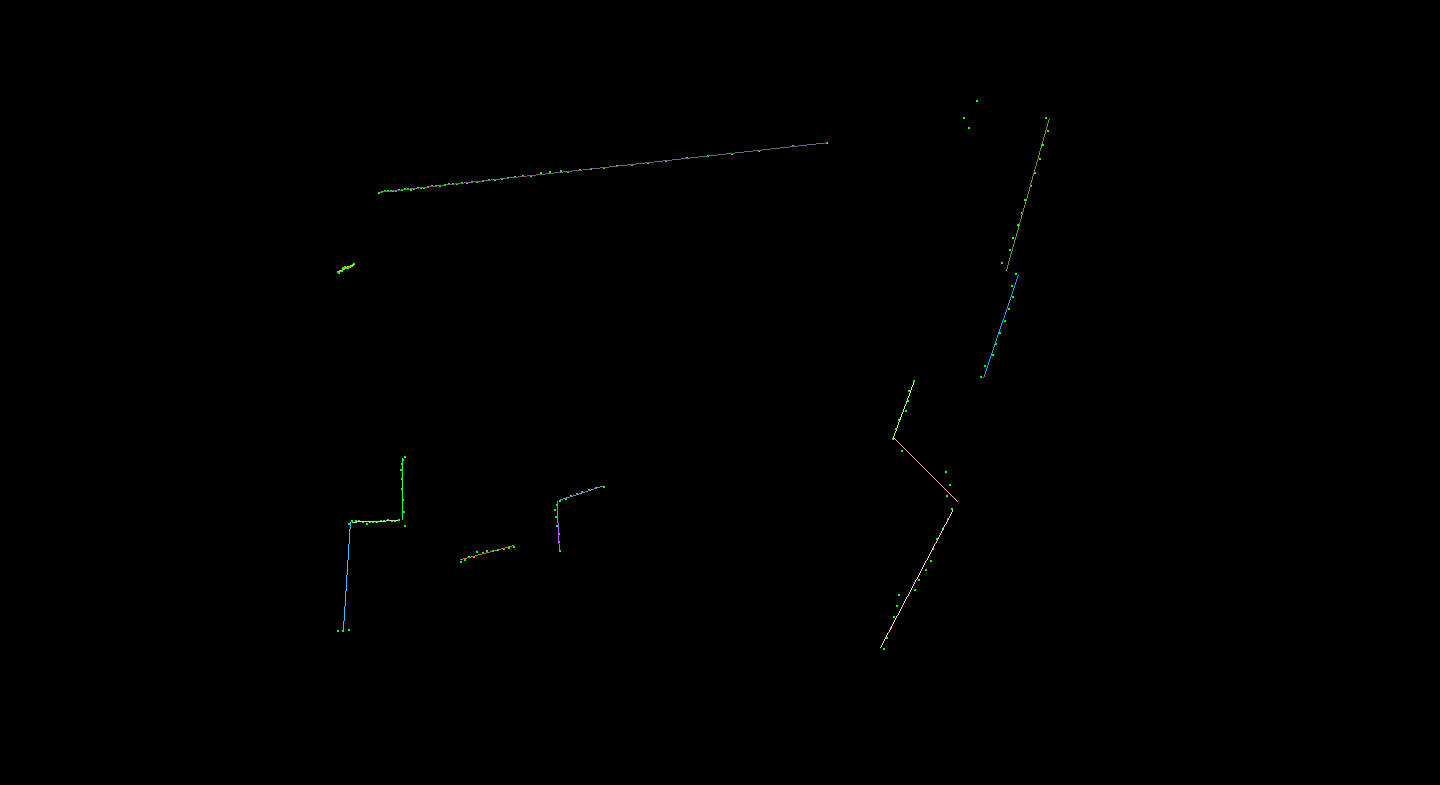
\includegraphics[width=0.7\textwidth]{figures/good_line_fit.png}
    \label{subfig:good_fit}
}
\subfigure[Bad example of line fits]{
    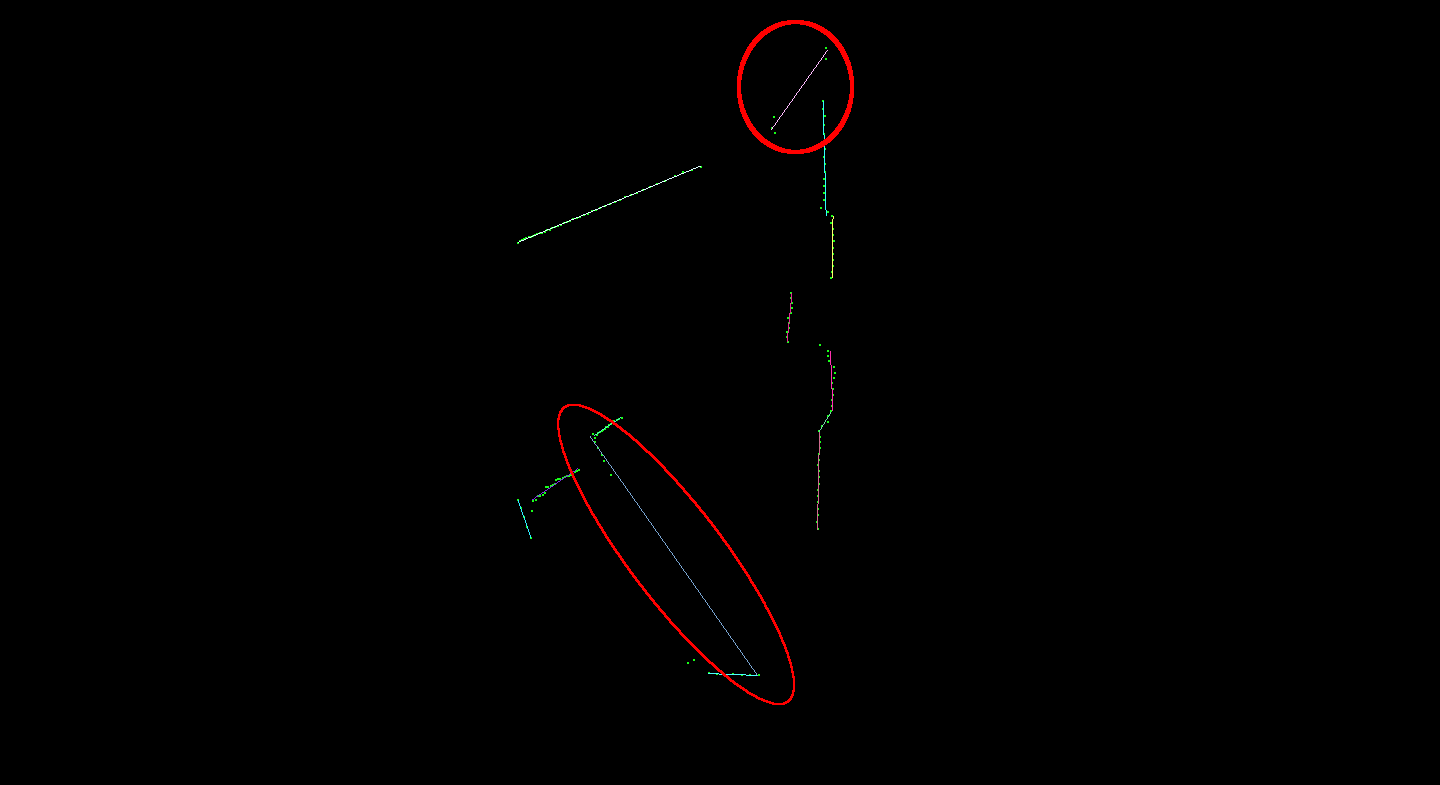
\includegraphics[width=0.7\textwidth]{figures/bad_line_fit_highlighted.png}
    \label{subfig:bad_fit}
}
\caption{Image~\subref{subfig:good_fit} shows a reasonable example of line fits
    extracted using agglomeration. Most lines are fit with quality similar to that
    seen here. However, some lines are fit poorly in cases where there are largeen
    discontinuities. For example, in \subref{subfig:bad_fit} we highlight a pair
    of fits we feel are bad. The line fit to the points in the upper corner, for
    example, is just being fit to two clusters of noise. There is no evidence
    that a line should exist, but the error in merges is small enough that it
    still gets through. The long, circled line starts out as a reasonable fit, but
    makes a large jump to an adjacent point where there is no evidence that such a
    connection should exist.
}
\label{fig:line_fits}
\end{figure}

\paragraph{C}
The idea is to weight fitting errors according to the probability that they came from sensor noise, as opposed to a bad fit. To do that, we project the covariance of the observation from $(r,\theta)$ space to $(x,y)$ and use its inverse as a weight factor in the MSE.

Let $p_i$ be an observation and $q$ a point on the line:

\[MSE = \sum{\left((p_i-q)^T\left(J\Sigma_zJ^T\right)^{-1}\hat{n}\right)^2} \]

Where $\hat{n}$ is a vector normal to the line, $\Sigma_z$ is the observation covariance in $(r,\theta)$ and $J$ is the jacobian of the function that maps observations in $(r,\theta)$ to the global $(x,y)$ coordinate frame.

This more principled model would make a significant difference when there is a lot of noise.  In this case the original MSE formula might not allow for points to be combined into a line because they are outside a given threshold.  This new calculation for MSE would weight down the seemingly large errors by taking into account that the large difference is more likely.
%% Task 3
\section{RANSAC Rigid-Body Transformation}

\paragraph{A}
Given a number of line correspondences, a set of 3 non-parallel lines that
intersect at unique locations would be sufficient to product a 2D RBT. To
compute the RBT, find the intersections of the lines in each set and then
use Horn's Algorithm to align the resulting sets of 3 points.

\paragraph{B}
Given a fit between lines in set A and lines in set B, we compute a RBT that
rotates A into B's space. To cheaply/quickly compute how good this fit is,
we discretize the world into bins and mark all bins that points from B fall
into. We then apply our transform to the points from A and see if they fall
into a bin from B. If so, we vote $1$, otherwise we vote $0$. The consensus
score is computed as the sum of votes. This is extremely fast as we only need
to bin the points in B once ever and checking for a hit by a point in A only
costs one transformation and a constant time check in a LUT.

After some tuning, we selected a bin size of 10\,cm. This seemed to be a good
balance between ensuring close fits and accounting for the fact that points do
not generally align exactly between scans.

\emph{Disclaimer: The use of a binning method for votes resulted from brainstorming with John Peterson,
    also in the class, about fast ways to calculate votes in such spaces since our existing methods
    were far too slow to use. We can not honestly claim completely that this idea is 100\% ours.}

\paragraph{C}
RANSAC makes good matches much of the time, provided the scans have a reasonable
amount of overlap. Fig.~\ref{fig:good_ransac0} shows how a translation of several
meters is still successfully found by RANSAC. However, eventually this may break
down, even in the presence of human-detectable features, more points will vote
for a bad alignment that ignores these ``good'' and result in the selection of
a sub-optimal transform. This is evident particularly in hallways, where straight,
parallel lines make up the majority of votes and, given the small amounts of overlap in
the optimal match, may vote for poor line matches that. Fig.~\ref{fig:bad_ransac0} gives
an excellent example of this. Finally, Fig.~\ref{fig:long_ransac} shows an example of
RANSAC finding the RBT for two scans that were separated by a significant amount
of travel. These scans were, in fact, of the same location and we were able to extract
a correct alignment from the data.

\begin{figure}[h!]
\centering
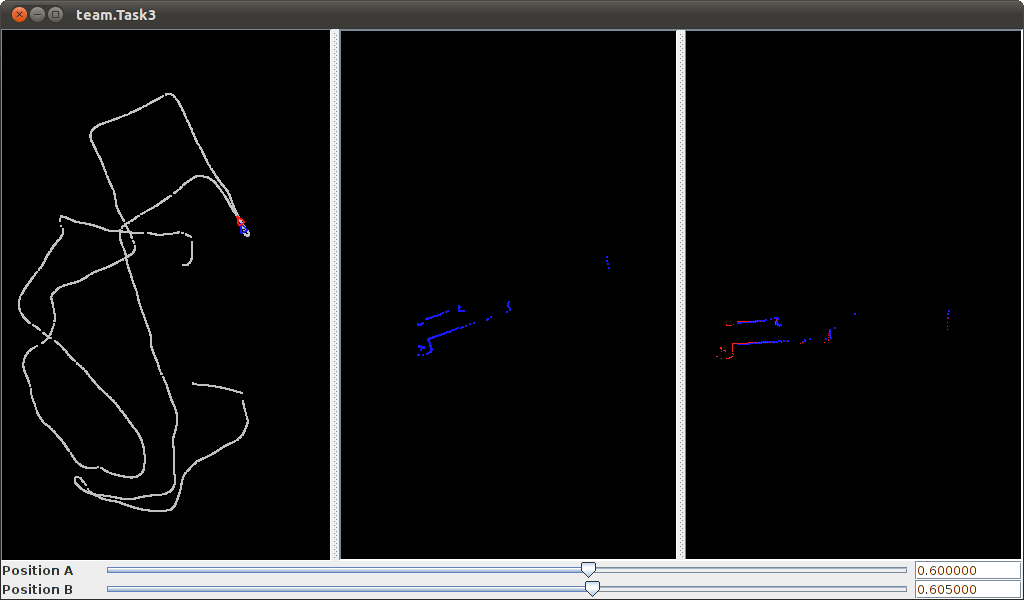
\includegraphics[width=.7\textwidth]{figures/Task3_good0.png}
\caption{A good scan match from RANSAC. Our implementation of RANSAC is able
to fit models to points that are translated or rotated by a non-negligible amount. As seen
in this figure, the recorded poses are separated by several meters, but RANSAC
was able to match features successfully.}
\label{fig:good_ransac0}
\end{figure}

\begin{figure}[h!]
\centering
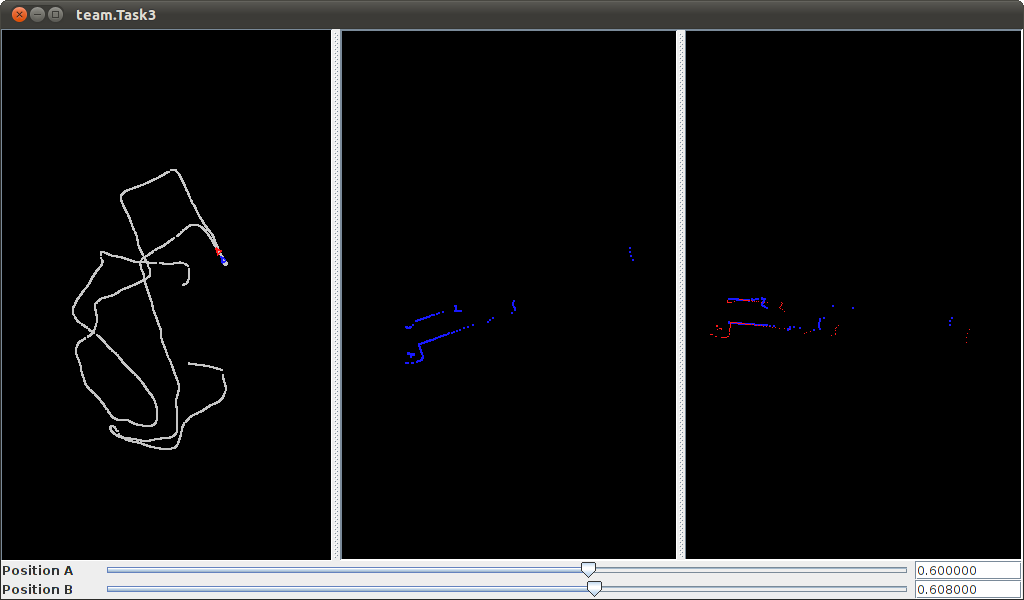
\includegraphics[width=.7\textwidth]{figures/Task3_bad0.png}
\caption{A bad scan match from RANSAC. Eventually RANSAC breaks down because the
    ``good'' features that a human can detect do not hold enough votes to outweigh
    less ``good'' matches. As seen in this figure, after moving the robot slightly
    down the hall from our previously shown good match, RANSAC breaks down and
    returns a significantly less reasonable transformation even though there are
    several features that indicate a good match is still possible.}
\label{fig:bad_ransac0}
\end{figure}

\begin{figure}[h!]
\centering
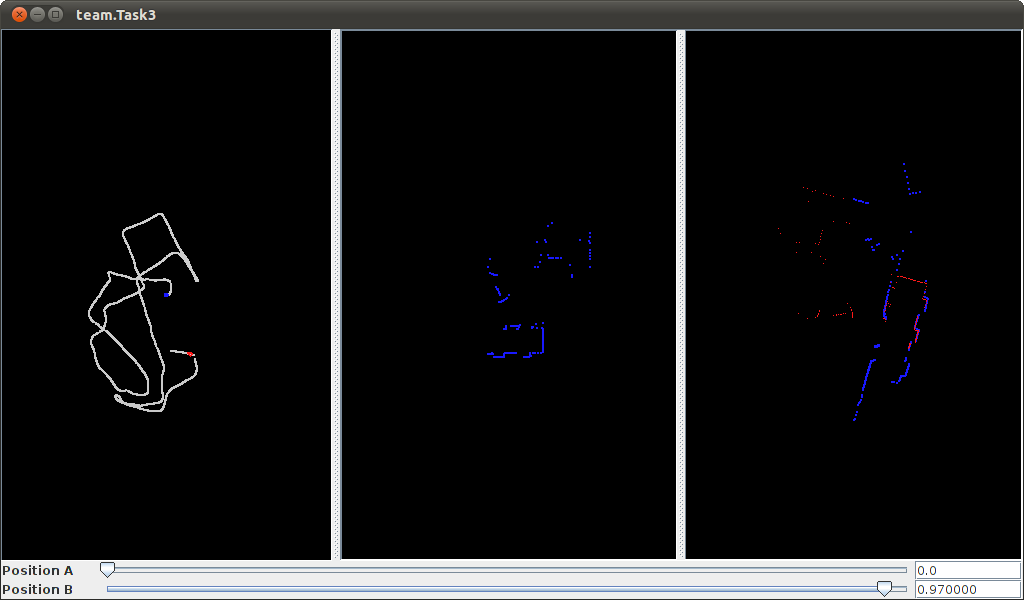
\includegraphics[width=.7\textwidth]{figures/Task3_good_endpoints.png}
\caption{A loop closure detected after significant travel. RANSAC is able to match
    scans when the robot returns to a familiar location after traveling a long
    distance. In this case, the robot starts in an elevator lobby and ends its
    travels in the same elevator lobby. RANSAC is able to detect this, providing a
    RBT that clearly matches the elevator lobby again, though from a different
    perspective.}
\label{fig:long_ransac}
\end{figure}
%% Task 4
\section{Advanced Data Association }
	Data association is the attempt to correlating observed features when we do
not have known data association.  Without good data association, SLAM won't work.
The three ways we have discussed doing data association in class are $\chi^2$
nearest neighbor, RANSAC, and JCBB.

	$\chi^2$ nearest neighbor %XXXX

	RANSAC uses random search to choose a model for associating
RANSAC is easy to implement and doesn't require points to be in any order since
it randomly selects them (however this means that it doesn't take advantage of points
that are ordered).  An additional advantage of RANSAC is that it can find associations
even when there are many outliers, if it is allowed to run long enough.  However, the
number of iterations to run, as well as the threshold used, change depending upon the
dataset.  A ``good" number of iterations can be calculated, but this doesn't guarantee
finding the best association since RANCAS is probabilistic. % XXX When would RANSAC be best

	JCBB seeks to create as few new features as possible (associate as many features
as it can) without surpassing a threshold.  It does this by intelligently searching a tree of
possible associations in which a newly observed feature can be associated with any
previously observed feature, and if none of these produce a $\chi^2$ less than a given
threshold the observation becomes a new feature.  It


%XXX The advantages of JCBB
\end{document}
